\section{Geradlinige Dreiecks Darstellungen (SLTRs)}

Ausgehend von den konvexen Einbettungen nach Tutte, kann man sich die Frage stellen unter welchen Vorraussetzungen wir einen planaren Graphen so zeichnen können, dass alle Gebiete Dreiecke umranden. Bei der Formalisierung dieser Darstellung und ersten Feststellungen halten wir uns an Nieke Aerts und Stefan Felsner \cite{af13,af15}.

\begin{definition}[SLTR]\label{defsltr}
Eine Zeichnung eines planen Graphen $G$ wird \textit{geradlinige Dreiecks Darstellung}, im weiteren kurz \textit{SLTR} (für die englische Bezeichnung \textit{staight line triangle representation}), genannt falls gilt:
\begin{itemize}
\item[S1] Alle Kanten sind Segmente von Geraden.
\item[S2] Alle Gebiete, inklusive dem Äusseren, sind nicht degenerierte Dreiecke.
\end{itemize}
\end{definition}

\begin{figure}[h]
	\centering
  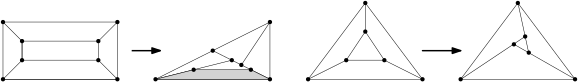
\includegraphics[width=0.9\textwidth]{sltr-example.png}
	\caption{Links einer der beiden 3-zusammenhängenden Graphen auf acht Knoten ohne SLTR und rechts ein Graph mit einer möglichen SLTR.}
\end{figure}

Um die Problemstellung greifbarer zu machen werden wir plane Graphen zusammen mit den Aufhängungen $\{a_1,a_2,a_3\}$ betrachten, wobei $\{a_1,a_2,a_3\}$ hier die designierten Ecken des äusseren Gebietes einer möglichen SLTR sind. Einen Graphen zusammen mit einem äusseren Gebiet bzw. festen Aufhängungen zu betrachten, macht auch in sofern Sinn, als dass planare Graphen existieren, von denen manche Einbettungen SLTRs zulassen, andere jedoch nicht, so wie in Abbildung \ref{10_example} zu sehen.

\begin{proposition}\cite[Proposition 1.2]{af13}
Sei $G$ ein planer Graph mit den Aufhängungen $\{a_1,a_2,a_3\}$ als äussere Ecken einer SLTR. Weiter gebe es keine inneren Knoten $v$ mit $deg(v) < 3$. Dann ist $G$ intern-3-zusammenhängend.
\end{proposition}

\begin{remark}
Für innere Knoten von Grad 2 in einer SLTR müssen beide angrenzenden Winkel gerade sein. Somit können wir diese Knoten durch eine gerade Kante zwischen ihren Nachbarn ersetzen und den resultierenden Graphen betrachten. Wir werden somit von nun an nur intern-3-zusammenhängende Graphen mit Aufhängungen betrachten, da alle anderen Graphen, die eine SLTR zulassen, auf diese reduziert werden können.
\end{remark}

\begin{figure}[h]
	\centering
  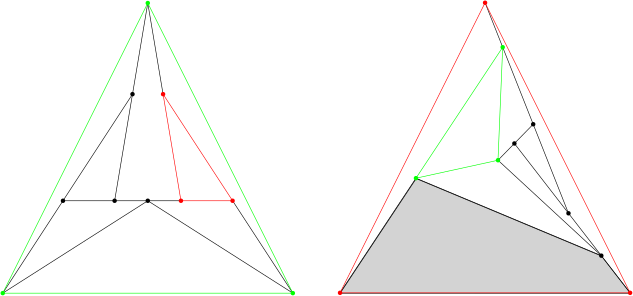
\includegraphics[scale=0.1]{10_example.png}
	\caption{Der kleinste 3-zusammenhängende kombinatorische Graph mit einer Wahl der Aufhängungen die eine SLTR zulässt und einer Auswahl ohne SLTR.}
	\label{10_example}
\end{figure}

Zu den Fragen, welche notwendigen und hinreichenden Bedingungen es für die Existenz von SLTRs gibt und  welche algorithmischen Ansätze es bei der Suche nach einer spezifischen Darstellung gibt haben Aerts und Felsner in \cite{af13}, \cite{af13h} und \cite{af15} schon einige Antworten geliefert, mit denen wir uns in den nächsten beidem Kapiteln beschäftigen werden. Zuerst müssen aber in diesem Kapitel noch ein paar notwendige Konzepte eingeführt werden.
